\clearpage
\newpage

\subsubsection{Estensione D: Modifica Rapida dello Stato delle Notifiche con Attivazione Immediata}

Questa variante rappresenta l’approccio duale dell’\textbf{Estensione C}, semplificando ulteriormente l’attivazione delle notifiche. L’obiettivo è ridurre i passaggi necessari per riattivare una categoria disattivata, mantenendo comunque un controllo chiaro sulla disattivazione.

\vspace{0.5cm}
\subsubsection{Interfaccia e Interazione}
Analogamente all’\textbf{Estensione C}, ogni categoria nella barra laterale dispone di un pulsante contestuale per modificarne lo stato. Il pulsante può assumere due stati:

\begin{itemize}
    \item \textbf{Attiva}, se la categoria è attualmente disabilitata.
    \item \textbf{Disattiva}, se la categoria è attualmente abilitata.
\end{itemize}

Le interazioni dell’utente variano a seconda dell’azione eseguita:

\begin{itemize}
    \item \textbf{Disattivazione di una categoria}:
    \begin{itemize}
        \item Al clic su \textbf{Disattiva}, appare un popup di conferma che informa l’utente sulle conseguenze della scelta, prevenendo azioni accidentali in linea con i principi di Nielsen \cite{nielsen1995}.
        \item Se confermata, la categoria viene spostata nella sezione delle notifiche disattivate tramite un’animazione di transizione.
        \item Il pulsante cambia stato, diventando \textbf{Attiva}, fornendo un feedback visivo chiaro sulla modifica.
    \end{itemize}
    
    \item \textbf{Attivazione di una categoria}:
    \begin{itemize}
        \item Al clic su \textbf{Attiva}, il sistema aggiorna immediatamente lo stato della notifica senza richiedere una conferma esplicita.
        \item La categoria viene spostata nella sezione delle notifiche attive con un’animazione fluida, applicando il principio della \textbf{gestalt della continuità} \cite{miller1956}.
        \item Il pulsante cambia stato in \textbf{Disattiva}, rendendo la modifica evidente e intuitiva.
    \end{itemize}
\end{itemize}

\subsubsection{Feedback Visivo e UX Design}
L’esperienza utente è ottimizzata tramite tecniche di design che garantiscono chiarezza e immediatezza:

\begin{itemize}
    \item \textbf{Popup di conferma per la disattivazione}: aiuta a prevenire errori e rende consapevole l’utente delle conseguenze della scelta \cite{nielsen1995}.
    \item \textbf{Animazione di transizione}: assicura una continuità visiva fluida nello spostamento delle categorie, migliorando la percezione del cambiamento \cite{miller1956}.
    \item \textbf{Aggiornamento immediato dello stato del pulsante}: il cambio di testo e colore riflette lo stato corrente della categoria, riducendo l’ambiguità e migliorando la prevedibilità dell’interazione.
\end{itemize}

Questa estensione semplifica l’attivazione delle notifiche, eliminando il passaggio della conferma e migliorando la fluidità dell’interazione, senza compromettere il controllo dell’utente sulla gestione delle proprie preferenze.

\begin{figure}[ht]
    \centering
    \begin{tikzpicture}[node distance=1.5cm and 1cm, auto]
        % Nodo per immagine 1 con didascalia sotto
        \node (img1) {
            \begin{tabular}{c}
                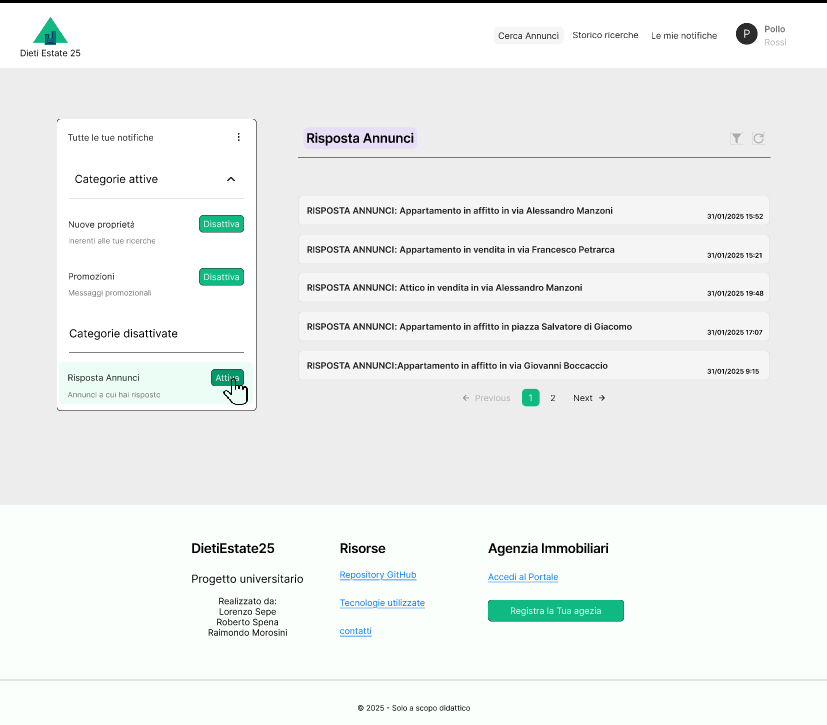
\includegraphics[width=0.6\textwidth]{Immagini/Mockup/notifiche/estensione D/clickAttiva.png} \\
                Cockburn: Extension D.2
            \end{tabular}
        };
        
        % Nodo per immagine 2 con didascalia sotto, posizionato a destra di img1
        \node (img2) [below=of img1] {
            \begin{tabular}{c}
                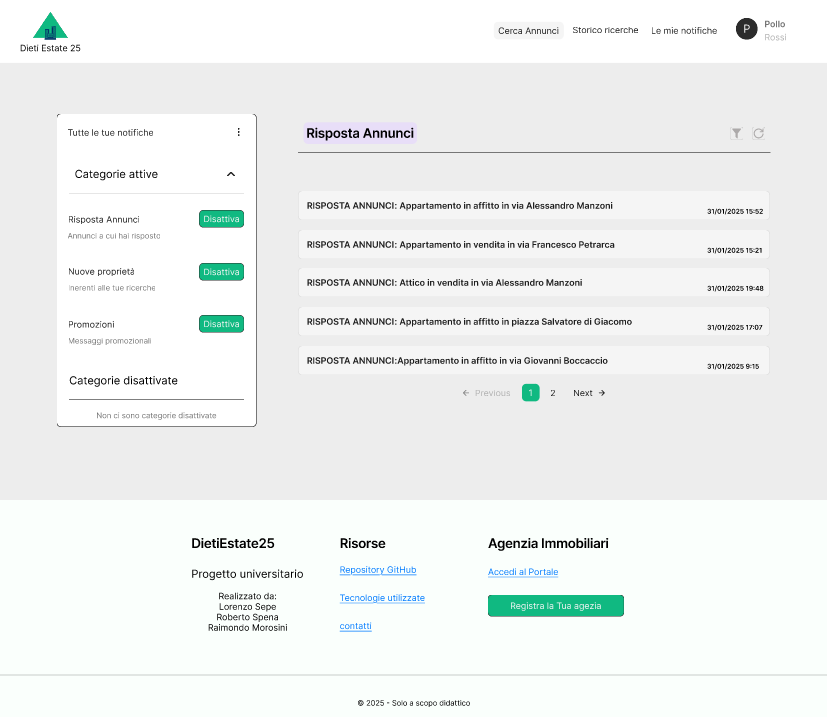
\includegraphics[width=0.6\textwidth]{Immagini/Mockup/notifiche/estensione D/attivato.png} \\
                Cockburn: step 8/9/10
            \end{tabular}
        };
        
        % Disegna le frecce
        \draw[->, thick] (img1) -- (img2);
      
    \end{tikzpicture}
    \caption{Mockup: estensione D della tabella di Cockburn del caso d'uso disattiva/attiva categoria notifica}
    \label{fig:tikz_flow}
\end{figure}

\newpage

